%% This file was auto-generated by IPython.
%% Conversion from the original notebook file:
%% svm2.ipynb
%%
\documentclass[11pt,english,fleqn]{article}

%% This is the automatic preamble used by IPython.  Note that it does *not*
%% include a documentclass declaration, that is added at runtime to the overall
%% document.

\usepackage{amsmath}
\usepackage{amssymb}
\usepackage{graphicx}
\usepackage{ucs}
\usepackage[utf8x]{inputenc}

% needed for markdown enumerations to work
\usepackage{enumerate}

% Slightly bigger margins than the latex defaults
\usepackage{geometry}
\geometry{verbose,tmargin=3cm,bmargin=3cm,lmargin=2.5cm,rmargin=2.5cm}

% Define a few colors for use in code, links and cell shading
\usepackage{color}
\definecolor{orange}{cmyk}{0,0.4,0.8,0.2}
\definecolor{darkorange}{rgb}{.71,0.21,0.01}
\definecolor{darkgreen}{rgb}{.12,.54,.11}
\definecolor{myteal}{rgb}{.26, .44, .56}
\definecolor{gray}{gray}{0.45}
\definecolor{lightgray}{gray}{.95}
\definecolor{mediumgray}{gray}{.8}
\definecolor{inputbackground}{rgb}{.95, .95, .85}
\definecolor{outputbackground}{rgb}{.95, .95, .95}
\definecolor{traceback}{rgb}{1, .95, .95}

% Framed environments for code cells (inputs, outputs, errors, ...).  The
% various uses of \unskip (or not) at the end were fine-tuned by hand, so don't
% randomly change them unless you're sure of the effect it will have.
\usepackage{framed}

% remove extraneous vertical space in boxes
\setlength\fboxsep{0pt}

% codecell is the whole input+output set of blocks that a Code cell can
% generate.

% TODO: unfortunately, it seems that using a framed codecell environment breaks
% the ability of the frames inside of it to be broken across pages.  This
% causes at least the problem of having lots of empty space at the bottom of
% pages as new frames are moved to the next page, and if a single frame is too
% long to fit on a page, will completely stop latex from compiling the
% document.  So unless we figure out a solution to this, we'll have to instead
% leave the codecell env. as empty.  I'm keeping the original codecell
% definition here (a thin vertical bar) for reference, in case we find a
% solution to the page break issue.

%% \newenvironment{codecell}{%
%%     \def\FrameCommand{\color{mediumgray} \vrule width 1pt \hspace{5pt}}%
%%    \MakeFramed{\vspace{-0.5em}}}
%%  {\unskip\endMakeFramed}

% For now, make this a no-op...
\newenvironment{codecell}{}

 \newenvironment{codeinput}{%
   \def\FrameCommand{\colorbox{inputbackground}}%
   \MakeFramed{\advance\hsize-\width \FrameRestore}}
 {\unskip\endMakeFramed}

\newenvironment{codeoutput}{%
   \def\FrameCommand{\colorbox{outputbackground}}%
   \vspace{-1.4em}
   \MakeFramed{\advance\hsize-\width \FrameRestore}}
 {\unskip\medskip\endMakeFramed}

\newenvironment{traceback}{%
   \def\FrameCommand{\colorbox{traceback}}%
   \MakeFramed{\advance\hsize-\width \FrameRestore}}
 {\endMakeFramed}

% Use and configure listings package for nicely formatted code
\usepackage{listingsutf8}
\lstset{
  language=python,
  inputencoding=utf8x,
  extendedchars=\true,
  aboveskip=\smallskipamount,
  belowskip=\smallskipamount,
  xleftmargin=2mm,
  breaklines=true,
  basicstyle=\small \ttfamily,
  showstringspaces=false,
  keywordstyle=\color{blue}\bfseries,
  commentstyle=\color{myteal},
  stringstyle=\color{darkgreen},
  identifierstyle=\color{darkorange},
  columns=fullflexible,  % tighter character kerning, like verb
}

% The hyperref package gives us a pdf with properly built
% internal navigation ('pdf bookmarks' for the table of contents,
% internal cross-reference links, web links for URLs, etc.)
\usepackage{hyperref}
\hypersetup{
  breaklinks=true,  % so long urls are correctly broken across lines
  colorlinks=true,
  urlcolor=blue,
  linkcolor=darkorange,
  citecolor=darkgreen,
  }

% hardcode size of all verbatim environments to be a bit smaller
\makeatletter 
\g@addto@macro\@verbatim\small\topsep=0.5em\partopsep=0pt
\makeatother 

% Prevent overflowing lines due to urls and other hard-to-break entities.
\sloppy

\setlength{\mathindent}{0pt}
\setlength{\parindent}{0pt}
\setlength{\parskip}{8pt}
\begin{document}

Destek Vektor Makinalari (Support Vector Machines) En basit halleriyle
SVM'ler risk minimize eden lineer siniflayicisidirlar.\[ R(\Theta) \leq J(\Theta) = R_{emp}(\Theta) +
\sqrt{ \frac{h \times (log(\frac{2N}{h}) + 1) - log(\frac{\eta}{4})}{N}}  \]
\textbf{h}: siniflayicinin kapasitesi

\textbf{N}: egitim verisinde kac veri noktasi oldugu

Vapnik ve Chernovenkis $1-\eta$ olasilikla ispaladi ki ustteki denklem
dogrudur. SVM algoritmasi hem $h$ degerini hem de sayisal, olcumsel
riski ayni anda minimize etmektedir, ve bunu sinir noktalarini
noktalarini ayirmakla yapmaktadir.

Turetelim

\begin{codecell}
\begin{codeinput}
\begin{lstlisting}
im=imread("svm-planes.png"); imshow(im)
\end{lstlisting}
\end{codeinput}
\begin{codeoutput}
\begin{verbatim}
<matplotlib.image.AxesImage at 0xae51f4c>
\end{verbatim}
\begin{center}
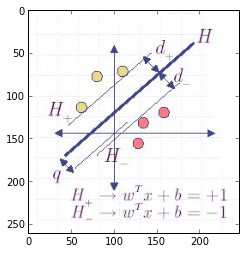
\includegraphics[width=0.7\textwidth]{svm2_files/svm2_fig_00.png}
\par
\end{center}
\end{codeoutput}
\end{codecell}
Karar duzlemi: $w^{T}x + b=0$

Soyle bir tanim yapalim: $q = min_{x}\big\|x - 0\big\|$

$q$, $H^{+}$ ve $H^{-}$ formullerini ileride kullanacagiz.

H icin: $q = min_{x}\big\|x - 0\big\|$ su sarta tabi $w^{T}x+b=0$

Lagrange: $min_{x}\frac{1}{2}\big\|x - 0\big\|^2+\lambda(w^{T}x+b)$

Gradyani alalim ($\frac{\partial}{\partial x}$) ve 0 degerine
esitleyelim.

Biraz cebirsel numaradan sonra: $q = \frac{|b|}{||w||}$

Tanim: $H^{+} = w^{T}x + b=+1$ $H^{-} = w^{T}x + b=-1$

Bu tanimi genellikte bir kayip olmadan yapabiliyoruz; $b$ \& $w$
degerlerini hala duzeltebiliriz.

$q^{+}$ ve $q^{-}$ degerlerinin hesapla

$q^{+} = \frac{|b-1|}{||w||}$

$q^{-} = \frac{|-b-1|}{||w||}$

Ayrac o zaman soyle

$m=q^{+}+q^{-} = \frac{|b-1-b-1|}{||w||} = \frac{|-2|}{||w||} = \frac{2}{||w||}$

Ayraclarin olabildigince ayirmasini istiyorsak $m$'i arttiriz (yani
$\frac{2}{||w||}$'i maksimize ederiz), ya da $||w||$ degerini minimize
ederiz.

Sinirlar

Veri noktalarini oyle siniflamak istiyoruz ki + ve - noktalar
hiperduzlemlerin dogru noktalarinda kalsinlar.
\[ w^{T}x+b \geq +1, \forall y_{i}=+1   \]\[ w^{T}x+b \leq -1, \forall y_{i}=-1  \]
Bu iki denklemi birlestirelim
\[ y_{i}(w^{T}x+b)-1 \geq 0  \]
Her seyi biraraya koyalim
\[ min \frac{1}{2}{||w||^2} \textrm{ subject to }  y_{i}(w^Tx_{i}+b)-1 \ge 0 \]
Bu form tanidik geliyor mu? Bu qp ile cozulebilecek karesel (quadratic)
bir formul, programdir!

qp

Python dilinde cvxopt paketi vardir Matlab Optimization Toolbox'da qp()
var. Steve Gunn'in SVM Toolbox'i icinde C ile yazilmis bir qp var
SVMLight icinde ayrica bir qp var qp fonksiyonlari problemleri genelde

$\frac{1}{2}x^{T}Px+q^{T}x$ formunda gormek isterler.

Biraz once elde ettigimiz denklemi bu istenen formata dogru
``masajlayabiliriz''

Ikiz (dual)

SVM ihtiyaclari icin ikiz formul (dual) ile calismak daha rahattir
Lagrange (tekrar) olusturalim, turevi alalim, ve sifira esitleyelim.
Bunun sonucunda elimize KKT noktalari gececektir

\begin{equation}L_{p} = \frac{1}{2}||w||^{2}-\sum_{i}\alpha_{i}(y_{i}(w^{T}x_{i}+b)-1)  \label{eq:primal}\end{equation}
\[ \frac{\partial}{\partial w} L_{p} = w-\sum_{i}\alpha_{i}y_{i}x_{i}=0  \]
\begin{equation}w = \sum_{i}\alpha_{i}y_{i}x_{i} \label{eq:wdual} \end{equation}

\begin{equation}
\frac{\partial}{\partial b} L_{p} = -\sum_{i}\alpha_{i}y_{i}=0  \label{eq:cdual}
\end{equation}

Ustteki iki denklemi asal (primal) denkleme koydugumuz zaman

\begin{equation}
\textrm{ Maksimize et } L_{D}=\sum_{i}\alpha_{i}-\frac{1}{2}\sum_{i}\sum_{j}\alpha_{i}\alpha_{j}y_{i}y_{j}x_{i}^{T}x_{j} \label{eq:svm}
\end{equation}

sinirlar
\[ \sum_{i}\alpha_{i}y_{i}=0  \]\[ \alpha_{i} \geq 0  \]
qp

Bu yine qp() formunda bir problem! Sadece bu sefer cozecegimiz
degiskenler $\alpha_i$'lar, $x$'lar degil. Ustteki denklem su forma
$\frac{1}{2}x^{T}Px+q^{T}x$ masajlanabilir Bunun yapmak icin
$P_{i,j}$'ye $-y_{i}y_{j}x_{i}^{T}x_{j}$ degerini atariz. Ve qp'yi
cagiririz Sonuc bir $\alpha$'lar listesi olacaktir.

$b$ degerini hesaplamak

KKT kosulunun sebebiyle sifir olmayan her $\alpha_{i}$ icin ana
problemde ona tekabul eden kisitlayici sart sıkıdır (tight), yani bir
esitliktir. O zaman sifir olmayan her $\alpha_{i}$ icin $b$'yi
$w^{T}x_{i}+b = y_{i}$ ifadesini kullanarak hesaplariz. Sifir olmayan
her $\alpha_{i}$'dan gelen $b$ yaklasik olarak diger other $b$'lere esit
olacaktir. Final $b$'yi hesaplamak icin tum $b$'lerin ortalamasini almak
numerik olarak daha garantidir.

Siniflayici Tamamlandi

Her yeni $x$ noktasi icin artik $sign(x^{T}w+b)$ ibaresini
siniflayicimiz olarak kullanabiliriz. $-1$ ya da $+1$ olarak geri
gelecek sonuc bize yeni noktanin hangi sinifa ait oldugunu
soyleyecektir.

Ornek Çıktı

\begin{codecell}
\begin{codeinput}
\begin{lstlisting}
im=imread("svmlinear.png"); imshow(im)
\end{lstlisting}
\end{codeinput}
\begin{codeoutput}
\begin{verbatim}
<matplotlib.image.AxesImage at 0xa7226ac>
\end{verbatim}
\begin{center}
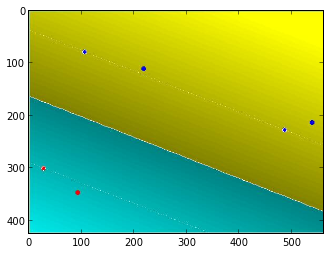
\includegraphics[width=0.7\textwidth]{svm2_files/svm2_fig_01.png}
\par
\end{center}
\end{codeoutput}
\end{codecell}
Cekirdekler (Kernels)

Simdiye kadar lineer ayraclardan bahsettik. SVM'ler lineer olmayan
ayraclarla da calisabilir. Cok basit: Bir temel fonksiyon kullanarak
girdiyi daha yuksek boyuta dogru bir onislemden gecirirsek bunu
basarabiliriz. Algoritmanin geri kalani degismeden kalacaktir.

Gayri Lineer Cekirdek

\begin{codecell}
\begin{codeinput}
\begin{lstlisting}
im=imread("svmpoly.png"); imshow(im)

\end{lstlisting}
\end{codeinput}
\begin{codeoutput}
\begin{verbatim}
<matplotlib.image.AxesImage at 0xa59ba2c>
\end{verbatim}
\begin{center}
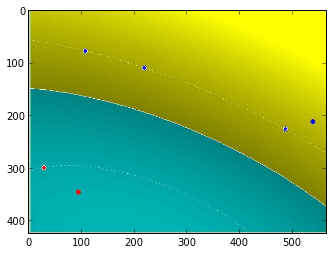
\includegraphics[width=0.7\textwidth]{svm2_files/svm2_fig_02.png}
\par
\end{center}
\end{codeoutput}
\end{codecell}
Esneme Payı Bazen bir problem ayrilmaya musait olmayabilir. Cok uc
noktalardaki bazi noktalar siniflayicinin calismasini imkansiz hale
getirebilir Bunun cozumu icin siniflayiciya ``esneme payı'' dahil
edebiliriz. Mesela $y_{i}=+1$ icin verinin yanlis tarafa dusmesini su
durumda izin verebiliriz: $w^{T}+b \geq -0.03$ Fakat eklemek gerekir ki
bu tur noktalarin ``cok fazla'' olmasini da istemiyoruz, bu sebeple bu
``yanlis'' noktalarin sayisina da bir ceza getirebiliriz.

\begin{codecell}
\begin{codeinput}
\begin{lstlisting}
from numpy import linalg
import cvxopt
import cvxopt.solvers

def svm(X, y):
    n_samples, n_features = X.shape

    # Gram matrix
    K = np.zeros((n_samples, n_samples))
    for i in range(n_samples):
        for j in range(n_samples):
            K[i,j] = np.dot(X[i], X[j])

    P = cvxopt.matrix(np.outer(y,y) * K)
    q = cvxopt.matrix(np.ones(n_samples) * -1)
    A = cvxopt.matrix(y, (1,n_samples))
    b = cvxopt.matrix(0.0)

    G = cvxopt.matrix(np.diag(np.ones(n_samples) * -1))
    h = cvxopt.matrix(np.zeros(n_samples))

    # solve QP problem
    solution = cvxopt.solvers.qp(P, q, G, h, A, b)

    print solution
    
    # Lagrange multipliers
    a = np.ravel(solution['x'])
    
    print "a", a

    # Support vectors have non zero lagrange multipliers
    ssv = a > 1e-5
    ind = np.arange(len(a))[ssv]
    a = a[ssv]
    sv = X[ssv]
    sv_y = y[ssv]
    print "%d support vectors out of %d points" % (len(a), n_samples)
    print "sv", sv
    print "sv_y", sv_y

    # Intercept
    b = 0
    for n in range(len(a)):
        b += sv_y[n]
        b -= np.sum(a * sv_y * K[ind[n],ssv])
    b /= len(a)
        
    # Weight vector
    w = np.zeros(n_features)
    for n in range(len(a)):
        w += a[n] * sv_y[n] * sv[n]

    print "a", a
    return w, b, sv_y, sv, a

X = np.array([[3.,3.],[4.,4.],[7.,7.],[8.,8.]])
y = np.array([1.,1.,-1.,-1.])
w, b, sv_y, sv, a = svm(X, y)
print "w", w
print "b", b
print 'test points'
print np.dot([2.,2.], w) + b # > 1
print np.dot([9.,9.], w) + b # < -1

\end{lstlisting}
\end{codeinput}
\begin{codeoutput}
\begin{verbatim}
pcost       dcost       gap    pres   dres
 0: -2.9061e-01 -5.0286e-01  6e+00  2e+00  1e+00
 1: -3.6857e-02 -3.0976e-01  3e-01  4e-16  1e-15
 2: -1.0255e-01 -1.2816e-01  3e-02  3e-17  7e-16
 3: -1.1074e-01 -1.1128e-01  5e-04  3e-17  7e-16
 4: -1.1111e-01 -1.1111e-01  5e-06  4e-17  7e-16
 5: -1.1111e-01 -1.1111e-01  5e-08  1e-17  6e-16
Optimal solution found.
{'status': 'optimal', 'dual slack': 7.403425105865883e-08, 'iterations': 5, 'relative gap': 4.79718822391507e-07, 'dual objective': -0.11111112756316754, 'gap': 5.330207369918724e-08, 'primal objective': -0.11111107426109389, 'primal slack': 2.7637512517768505e-08, 's': <4x1 matrix, tc='d'>, 'primal infeasibility': 1.077377601559697e-17, 'dual infeasibility': 6.043668397566901e-16, 'y': <1x1 matrix, tc='d'>, 'x': <4x1 matrix, tc='d'>, 'z': <4x1 matrix, tc='d'>}
a [  2.76375125e-08   1.11111073e-01   1.11111073e-01   2.76375125e-08]
2 support vectors out of 4 points
sv [[ 4.  4.]
 [ 7.  7.]]
sv_y [ 1. -1.]
a [ 0.11111107  0.11111107]
w [-0.33333322 -0.33333322]
b 3.66666541806
test points
2.33333253877
-2.33333253877
\end{verbatim}
\end{codeoutput}
\end{codecell}
Not: Ikizdeki $L_d$'yi maksimize ediyoruz, fakat hala qp()'deki minimize
ediciyi cagiriyoruz. Bu sebeple tum $\alpha$'larin toplamini temsil eden
$q$'larin negatifini aliyoruz, np.ones(n\_samples) *-1 isleminde
goruldugu gibi. Formuldeki karesel kisim icinde zaten $-\frac{1}{2}$
negatif ibaresi var, boylece geri kalan formulun degismesine gerek yok.

Kaynaklar

http://www.mblondel.org/journal/2010/09/19/support-vector-machines-in-python

Jebara, T., Machine Learning Lecture, Columbia University

\end{document}
